\section{The Meaning Model}\label{sec:model}

% But the LLM is not an agent -- certainly not an intentional one. Rather, LLMs really are much like the mythic figure of the oracle. The prophecies from Delphi were often incoherent and always cryptic; yet they were still \textit{meant}. And insofar as meaning is what we are concerned with, models mean. And in reality, humans are very much like this too -- the veneer of intentionality masks a continual self-constitution \citep{Lonergan:CognitionalStructure}.

The LLM is both a social-material object and a meaning-agent.
It is natural to ask why a model can be considered a meaning-agent -- we do not explore this here, but instead in $\S$\ref{appendix:possibility}.
Humans inscribe the LLM as a social-material object. In this process, the formal structure of the statistical intelligibility in language \citep{doi:10.1080/00437956.1954.11659520, Lonergan:Insight} is inscribed into a statistical machine -- the LLM. At an abstract level, this is very similar to how language itself captures the intelligibility of the world. Other similar examples form cornerstone human cultural technologies \citep{YiuGopnik:CulturalTechnologies}. In this sense, a latent LLM is an object for humans. But an LLM, once activated, becomes something more: a meaning-agent \cite{Arcas:MachinesBehave}. We will proceed to explore this process. In so doing, we go from the model as a scientific object to apprehending the model in experience, reading the objectivity of the model as textual \citep{Hegel:PhG, Gadamer:TruthAndMethod, Heidegger:BeingAndTime}. 

%\subsection{Hermeneutics of model architecture}\label{sec:model:architecture}

\begin{figure}
     \centering
     \begin{subfigure}{0.45\linewidth}
         \centering
         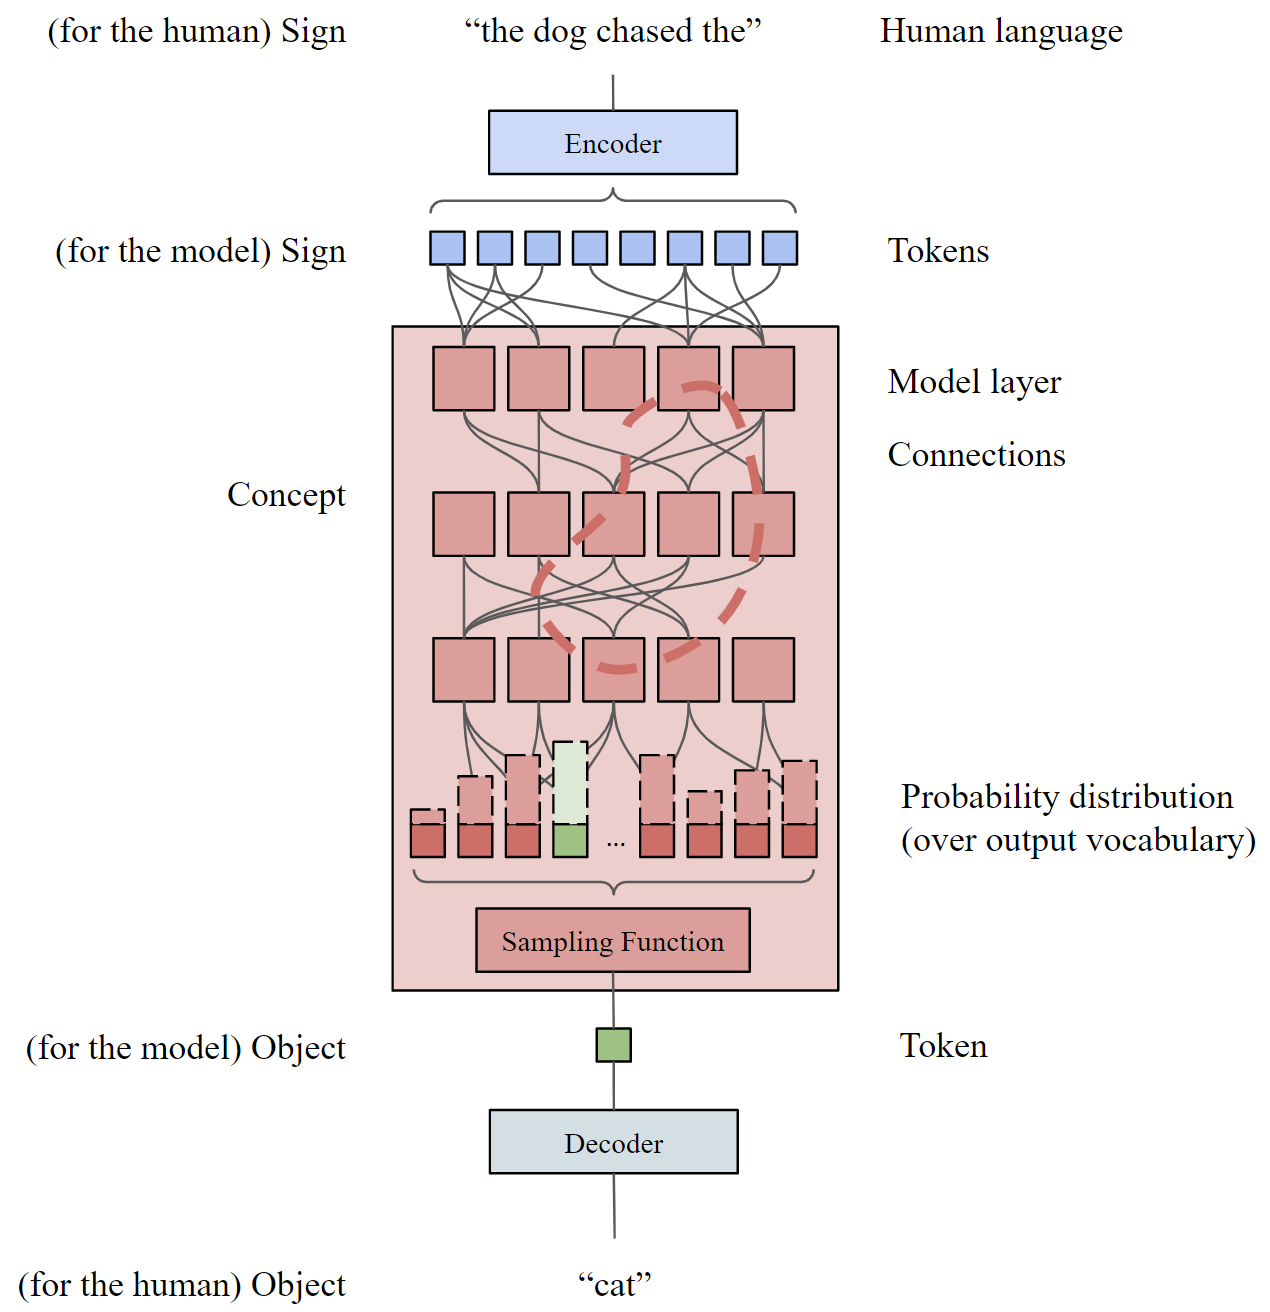
\includegraphics[height=7cm]{NeurIPS/imgs/inscription8.png}         \caption{\raggedright{\textit{Inscription.} A forward-pass mediates the picking-out of an object from a sign.}}
         \label{fig:inscription}
     \end{subfigure}
     % \hfill
     \hspace{2mm}
     \begin{subfigure}{0.45\linewidth}
         \centering
         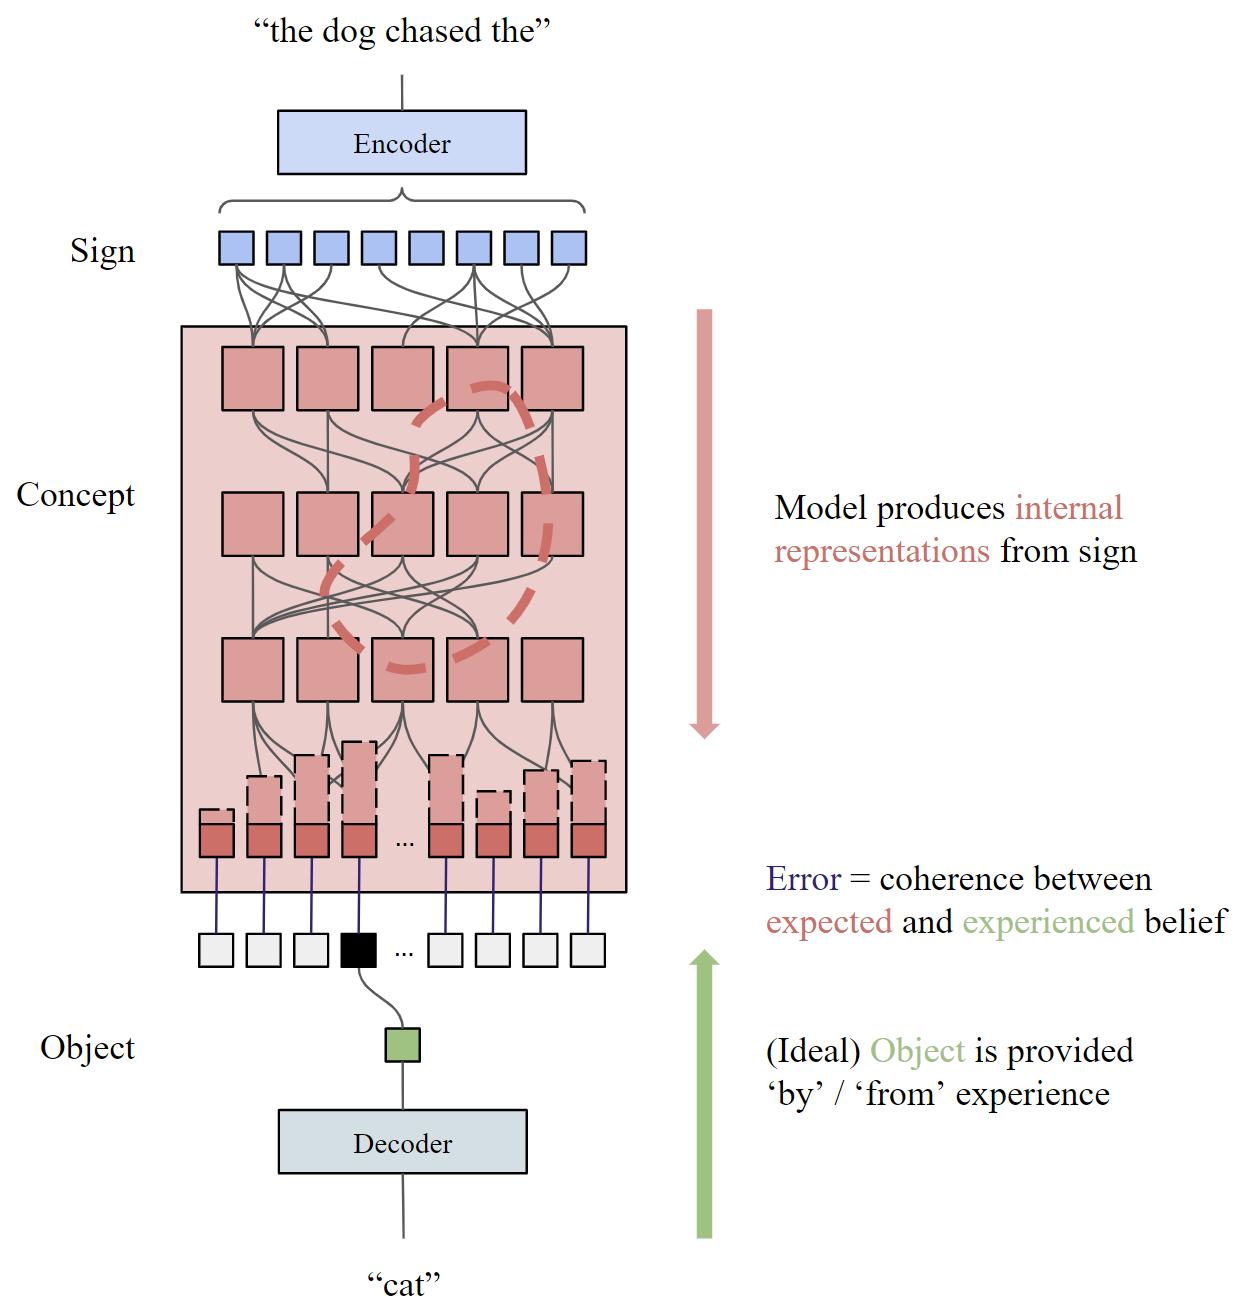
\includegraphics[height=7cm]{NeurIPS/imgs/shithishihtihi.png}
         \caption{\textit{Concretization.} Backpropagation adjusts model concepts in response to error.}
         \label{fig:reification}
     \end{subfigure}
     
    \caption{Inscription and concretization represented in LLMs. See $\S$\ref{sec:model} for a more thorough exploration.}
    \label{fig:conc_inscrip}
\end{figure}

%Now, we provide a technical reading of LLMs through the general theory of meaning. 
An LLM $f$ is a function from a variable-length sequence of tokens $\vec x = \{ x_1, ..., x_n \}$ to a single token $\hat{y}$.\footnote{Although this may be for next-token prediction, it also applies to schemes like self-supervised masked token prediction which do not observe a strictly sequential relationship.}
By this definition, the sampling procedure which selects a particular token from a probabilistic distribution over the output vocabulary is part of the LLM; different sampling procedures produce different output tokens.
\textbf{The LLM is a repository for concepts which are activated by the sign $\vec x$ to pick out the object $\hat{y}$. }
The sign and object are of the same substance; they are all tokens in the model's ``phenomenal world'', such that the model may encounter an object as a sign.
Autoregressive generation, for instance, is a series of operations $\{x_1, ..., x_p\} \to_f \hat{y}_1, \{x_1, ..., x_p, \hat{y}_1 \} \to_f \hat{y}_2, ... \{x_1, ..., x_p, ..., \hat{y}_{n-1}\} \to_f \hat{y}_n$.
In this case, the model encounters the object of its world which it has previously picked out as part of the sign in another operation.
Empirical work in model interpretability demonstrates that LLMs and neural networks of sufficient scale generally develop concentrations of features developed from statistical co-occurrences throughout training~\citep{Frankle2018TheLT,Kauffmann2019FromCT,Zhang2020ASO}. These concentrations represent the models' concepts.
% \textcolor{red}{Need to cite these studies.}

In LLMs, \textit{concretization} corresponds to weight update during training~(\ref{fig:reification}). At each timestep in training, the following steps are observed.
First, a pair $\langle \vec x, y \rangle$ is retrieved from the training dataset, where $y$ is the ``ground truth'' token.
Second, the model performs a \textit{partial} forward pass to obtain the probability distribution over the output vocabulary $\vec{p}$. 
Third, the difference between $\vec{p}$ and $y$ is computed as the error (encoding $y$ to make the computation feasible). 
Fourth, this error is propagated back throughout the model such that on another such partial forward pass the error would have been smaller.
During training, the model is repeatedly presented with co-occurrences of sign and object. Accordingly, the model develops internal clusters of representations (\textit{concepts}), thereby undergoing \textit{concretization}.
On the other hand, \textit{inscription} corresponds to inference $\vec x \to_f \hat{y}$, in which the model writes back `into the world' such that it may potentially encounter it again (for instance, in autoregressive generation)~(\ref{fig:inscription}).
This strict separation between concretization and inscription is in stark contrast to their intertwinedness for humans.
%\jared{We should say something like. Note the strict separation between inscription and reification in LLMs. That's different!}
However, the observed phenomenon that LLM-generated content is increasingly infiltrating datasets used to train LLMs~\citep{Shumailov:Curse} is an instance of inscription and concretization simultaneously at work.

